\documentclass[11pt]{article}
\usepackage[utf8]{inputenc}
\usepackage[myheadings]{fullpage}
\DeclareUnicodeCharacter{0301}{\hspace{-1ex}\'{ }}

% Package for headers 
\usepackage{fancyhdr}
\usepackage{lastpage}
\usepackage{pdfpages}

% For figures and stuff
\usepackage{graphicx, wrapfig, subcaption, setspace, booktabs}
\usepackage[T1]{fontenc}

% For lists
\usepackage{enumitem}
\usepackage{booktabs}

% Change for different font sizes and families
\usepackage[font=small, labelfont=bf]{caption}
\usepackage{fourier}
\usepackage[protrusion=true, expansion=true]{microtype}
\usepackage{url}

% Maths
\usepackage{amsmath,amssymb}
\usepackage{float}
\usepackage{graphicx}
\usepackage{wrapfig}
\usepackage[colorinlistoftodos]{todonotes}
\usepackage[colorlinks=true, allcolors=blue]{hyperref}

% For python code
\usepackage{color} 
\usepackage{listings} 
\usepackage{setspace} 

\definecolor{Code}{rgb}{0,0,0} 
\definecolor{Decorators}{rgb}{0.5,0.5,0.5} 
\definecolor{Numbers}{rgb}{0.5,0,0} 
\definecolor{MatchingBrackets}{rgb}{0.25,0.5,0.5} 
\definecolor{Keywords}{rgb}{0,0,1} 
\definecolor{self}{rgb}{0,0,0} 
\definecolor{Strings}{rgb}{0,0.63,0} 
\definecolor{Comments}{rgb}{0,0.63,1} 
\definecolor{Backquotes}{rgb}{0,0,0} 
\definecolor{Classname}{rgb}{0,0,0} 
\definecolor{FunctionName}{rgb}{0,0,0} 
\definecolor{Operators}{rgb}{0,0,0} 
\definecolor{Background}{rgb}{0.98,0.98,0.98} 
 
\lstdefinelanguage{Python}{ 
  numbers=left, 
  numberstyle=\footnotesize, 
  numbersep=1em, 
  xleftmargin=1em, 
  framextopmargin=2em, 
  framexbottommargin=2em, 
  showspaces=false, 
  showtabs=false, 
  showstringspaces=false, 
  frame=l, 
  tabsize=4,
  % Basic 
  basicstyle=\ttfamily\small\setstretch{1}, 
  backgroundcolor=\color{Background}, 
  % Comments 
  commentstyle=\color{Comments}\slshape, 
  % Strings 
  stringstyle=\color{Strings}, 
  morecomment=[s][\color{Strings}]{"""}{"""}, 
  morecomment=[s][\color{Strings}]{'''}{'''}, 
  % keywords 
  morekeywords={import,from,class,def,for,while,if,is,in,elif,else,not,and,or,print,break,continue,return,True,False,None,access,as,,del,except,exec,finally,global,import,lambda,pass,print,raise,try,assert}, 
  keywordstyle={\color{Keywords}\bfseries}, 
  % additional keywords 
  morekeywords={[2]@invariant,pylab,numpy,np,scipy}, 
  keywordstyle={[2]\color{Decorators}\slshape}, 
  emph={self}, 
  emphstyle={\color{self}\slshape}, 
  % 
} 
 
\linespread{1.3}


% Bibliography
% \usepackage{biblatex}
\usepackage{natbib} 
% \addbibresource{references.bib}

%% Language and font encodings
\usepackage[english]{babel}
\usepackage{csquotes}
\usepackage{todonotes}


\newcommand{\HRule}[1]{\rule{\linewidth}{#1}}
\onehalfspacing
\setcounter{tocdepth}{5}
\setcounter{secnumdepth}{5}

%% Sets page size and margins
\usepackage[a4paper,top=2cm,bottom=1.5cm,left=2cm,right=2cm,marginparwidth=1.5cm]{geometry}

\pagestyle{fancy}
\fancyhf{}

% Header and footer information
\setlength\headheight{15pt}
% \fancyhead[L]{s1000000} 
\fancyhead[R]{B. Klein Ikkink}
\fancyfoot[R]{\thepage}
 \setlength {\marginparwidth }{2cm}

\begin{document}

\date{}

% Do not change anything here except in \LARGE \textbf{This is the title of the essay} 
% /hline before and after the title makes those horoziontal lines appear, you can change the appearance by changing the 2pt to different sizees
\title{ \normalsize Engineering Physics, The Hague University of Applied Sciences, Delft
		\\ [1.0cm]
		% Change to your faculty if needed
		
\includegraphics[width=100mm]{img/cover/hhs_en_groen_hex.png}  %\\[.5cm]
		%and   \\[.5cm]
		%\includegraphics[width=50mm]{img/company_Logo.png}\\[.5cm]
		%\normalsize Company Name \\ [1.0cm]
		%Faculty of Social Sciences\\
		\HRule{2pt} \\
		\LARGE \textbf{Remote-controlled fabrication of 2D heterostructuren} %para que quede encerrado en las lineas
		\HRule{2pt} \\ [0.5cm]
		\normalsize \today \vspace*{5\baselineskip}}
		
\date{}

\author{
        Report by:\\
		B. Klein Ikkink            \\[1cm]
		 Supervised by:        \\
		 S. Bhattacharyya, LION \\
		 F. Galli, LION \\
		 }
		 
\maketitle
\pagenumbering{roman}

\clearpage
\section*{Foreword}
\todo{Add the foreword}
\clearpage

\section*{Abstract}
\todo{Create the abstract}
\clearpage

\newpage

\tableofcontents
\newpage

\section*{Used abbreviations}
\label{ap:veel_gebruikte_symbolen}
\todo{pagina nummering pas hier beginnen, voorgaande in romeinse nummering}
\begin{itemize}[noitemsep]
    \item LION : Leiden Institute Of Physics
    \item VDWSF: Van Der Waals Stacking Facility
    \item FMD : Fine Mechanical Department
    \item ELD : Electronics Department
    \item TUI : Terminal User Interface (differend from CLI in the sense that the user doesn't directly interact with the command line)
    \item GUI : Graphical User Interface
    \item SDK : Software Development Kit
    \item DAS : Domain Applied Science

\end{itemize}

\clearpage
\pagenumbering{arabic}

\section{Introduction}
\todo{Rephrase the text so it isn't flagged as plagiaat}
The discovery of graphene in 2004, awarded the Nobel Prize in Physics in 2010, has led to a completely new field of research based on 'atomically thin materials', materials of a few atomic layers thick (2D materials). 
Recently, the focus of the research area has shifted to fabricating completely new structures by stacking different atomically thin materials 'Van Der Waals Heterostructures'. 
Atomic thin materials can consist of metals, semiconductors, insulators, ferromagnets, superconductors, etc., combining these materials is a route to developing useful devices \citep{geimVanWaalsHeterostructures2013}. \\

Recently, a new research group was started under Principle Investigator Dr. Semonti Bhattacharyya who is an expert in fabricating and characterizing Van Der Waals Heterostructures and 2D materials and who recently started her new laboratory at LION, the Van Der Waals Stacking Facility (VDWSF).
This project will focus on the efficient and accurate fabrication and imaging of the Van Der Waals Heterostructures and will be carried out by the Van Der Waals stacking lab at the Leiden Institute of Physics (LION). 
LION is one of the oldest physics research institutes in the Netherlands. 
The research performed at Leiden Institute of Physics covers a broad spectrum of topics, from cosmology to condensed matter physics, from quantum computers to new systems such as Van Der Waals Heterostacks.
Research at LION is largely fundamental and curiosity-driven but also with an eye toward societal value. \\

This project will take place at the Leiden Institute of Physics (LION), which is one of the oldest physics institutes in the Netherlands.
Research at the Leiden Institute of Physics covers a broad spectrum of subjects, ranging from cosmology to condensed matter physics, from the physics of jamming in granular materials to quantum computation, from protein folding to superconductivity and novel systems like van der
Waals materials. 
Recently a new research group has been appointed to Semonti Bhattacharyya who is an expert in fabrication and characterisation of van der Waals and 2D materials and who has recently started to setup her new laboratory at LION, the Van Der Waals Stacking Facility (VDWSF). This project will focus on the efficient and accurate fabrication and imaging of the Van Der Waals Heterostructures with adaptability in mind to make the instrument more flexible and fit future research projects.


\clearpage
\section{Project definition}
\noindent Presently a commercial setup for fabricating 2D Hetero-stacks is used in the Van Der Waals Stacking Facility (VDWS) at lion. 
This commercial setup is prone to vibrations and has an inferior-quality microscope, wich makes it difficult to clearly identify small 2D material.
Furthermore, the laboratory has a vibration level slightly above VC-C \citep{isolationVibrationCriterionVC}.
For these reasons a new setup will be developed that should be less sensitive to mechanical vibrations.
This setup is focused on improved rigidity, accuracy and flexibility compared to the commercially available and previous versions.
The setup will be based on a commercial (Olympus BXFM) optical microscope, but to reach this goal a custom microscope stand, sample holder, mask holder and software have to be developed.

\subsection{Research question}
\begin{center}
    \textit{What components and control techniques should be used to make the stacking setup as least susceptible to vibration as possible and controllable at the sub-micrometer scale while producing clear images with an optical microscope?}
\end{center}

\subsection{Research goal}
\begin{center}
    \textit{Building a stacking setup that is as least susceptible to vibration as possible where the base x-y-z stages move with resolution on the micrometer scale and the mask x-y-z stages on the nanometer scale, which can be remotely controlled, while being able to capture clear images with an optical microscope.}
\end{center}

\clearpage

\section{Background}
Over the past decade, research into two-dimensional (2D) materials and van der Waals heterostructures has opened up a world of possibilities for the development of new technologies. 2D materials, such as graphene and hexagonal boron nitride, are atomically thin and have unique electrical, optical, and mechanical properties that make them interesting for a variety of applications.

\subsection{van der Waals Heterostuctures}

\todo{citaat invoegen}
\todo{aFBEELDING VAN GRAFEEN EN HEXAGONAAL BOORNITRIDE INVOEGEN}
Van der Waals heterostructures are composed of two or more 2D materials that are stacked together and can be used to create electronic and optoelectronic nano devices. 
This research has enabled the development of a wide range of technologies, including flexible electronics, high-speed transistors, and ultra-sensitive sensors. 
The promise of 2D materials and van der Waals heterostructures is that they can be used to create devices that are faster, more efficient, and more reliable than existing technologies \citep{geimVanWaalsHeterostructures2013}.

 \subsection{Fabrication of van der Waals Heterostructures: Stamping}
 The stamping process is a method used to fabricate van der Waals heterostructures.
 This process involves the transfer of 2D crystals onto a substrate by pressing them together with a stamp so the van der Waals forces between the layers become strong enough to hold the layers together.

 The general stamping procedure is as follows:
 \begin{enumerate}[noitemsep]
  \item The 2D material flakes are plased on top of the substrate
  \item The operator looks for suitable flakes to use for the stamping
  \item The operator places the stamp on top of the 2D material flake and changes the sample temperature to stick the flake to the stamp
  \item The stamp with the flake is positioned above the second 2D material flake on the substrate
  \item The operator places the stamp on top of the second 2D material flake and changes the sample temperature to release the flake from the stamp
  \item The operator finds a new suitable flake to place on top of the created stack and repeats the process
 \end{enumerate}

 This process consists of serval time consuming steps, such as finding suitable flakes, placing the flakes on the stamp and substrate, and changing the sample temperature.
 The aim of this project is to automate the process of stamping to reduce the time needed to fabricate a stack and to increase the accuracy of the process.

\subsection{Vibration isolation}
Bij het ontwerpen van de stand van de microscoop moet sterk rekening gehouden worden met de rigiditeit en eigenfrequensie van de opstelling. 
Bij commercieel verkrijgkbare stacking opstellingen is een faseverschil tussen trilling door het monster, masker en camera een bekend en veel voorkomend probleem, dit heeft als effect dat de uitlijning van flakes en het stapelen bemoeilijkt worden en de kans op beschadigen van de flake aanzienlijk groter is.

\todo{Stuk invoegen over verandering in fase plot (bode) bij verschillende massa, hoe hoger de massa hoe verder de fase drop naar beneden schuift, alles boven de grens heeft geen onvloed op de opstelling}
\todo{Grafiek maken van harmonische response over tijd van de gemaakte overdrachtsfunctie (zou alleen bij lage f met hoge A in trilling moeten komen.}

Het doel van het in house fabriceren van de microscoop stand is dan ook het behalen va een betere performance op het gebied van trillingsisolatie en rigiditeit tegenover commercieel verkrijgbare standaarden.

Bij het bestuderen van trillings respons van een opstelling kan er gekeken worden naar kracht gedreven trilling (er word een periodieke kracht uitgeoefend op een vast punt op het instrument) of er kan gekeken worden naar amplitude gedreven trilling (trillen van het oppervlak onder het instrument).
Het is belangrijk om het onderscheid tussen beide methodes te maken omdat deze wiskundig verschillend worden beschreven en ook anders dynamisch gedrag vertonen \citep{hesselberthBasicCalculationsVibration2015}, in het geval van dit project zal er gekeken worden naar een sterk gesimplificeerd model voor een amplitude gedreven trilling (zie figuur \ref{fig:1DOFoscilator}.

\begin{figure}[H]
  \centering
  \begin{minipage}[b]{0.30\textwidth}
    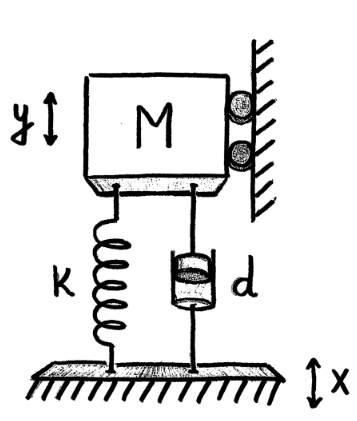
\includegraphics[width=\textwidth]{img/resonance/simplified_1DOF_oscilator.png}
    \caption{Schematic of a simplified microscope as a mass spring dampener system on a vibrating base. \citep{hesselberthMicroscopieBeweging}}
    \label{fig:1DOFoscilator}
  \end{minipage}
  \hfill
  \begin{minipage}[b]{0.65\textwidth}
    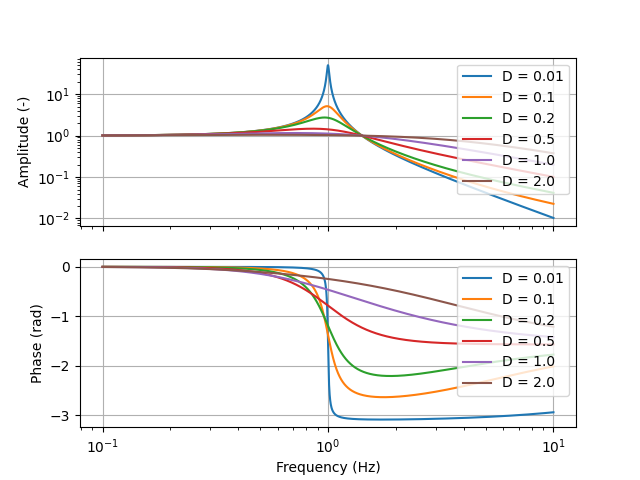
\includegraphics[width=\textwidth]{img/resonance/bode_plot_w01.png}
    \caption{}
    \label{fig:amp_driven_bode}
  \end{minipage}
\end{figure}

Door de opstelling te zien als een gedempt massa veer system (zie figuur \ref{fig:1DOFoscilator})kan met regeltechniek theorie het verwachte dynamische gedrag benadert worden. 
Om de berekeningen te versimpelen word de opstelling verdeelt in 2 inertiaalsetelsels, stelsel $Y$ met coorinaat $y$ voor de uitwijking van de massa $m$ met respect tot de evenwichtspositie van de massa en $X$ met coordinaat $x$ voor de uitwijking van de basis met respect tot de evenwichtspositie.
Omdat het gedrag als functie van tijd voor dit systeem niet van belang alleen de overdracht als functie van frequenstie kan er gekeken worden naar de overdracht van het systeem in het Laplace domein.
Het model bestaat uit de gecombineerde krachten balans in de Z richting zoals beschreven in formule \ref{eq:krachten balans instrument}.
Door de balans vervolgens te transformeren naar het Laplace domein en te herordenen kan de overdrachtsfunctie zoals beschreven in formule \ref{eq:trilling overdracht met demping} verkregen worden.

\begin{equation}
    m \frac{\mathrm{d}^2 y}{\mathrm{d} t^2} + d \frac{\mathrm{d}y}{\mathrm{d}t} +ky = d\frac{\mathrm{d}x}{\mathrm{d}t} + kx
    \label{eq:krachten balans instrument}
\end{equation}

\begin{equation}
    \omega_0 = \sqrt{\frac{k}{m}}; \quad D = \frac{d}{\sqrt{2mk}}; \quad f = \frac{\omega}{\omega_0}
\end{equation}

\begin{equation}
    H = \frac{Y}{X} = \frac{dj\omega + k}{-m\omega^2 +dj\omega + k} = \frac{\omega_0^2 + 2jD\omega_0^2 f}{\omega_0^2 + 2jD\omega_o^2 f - \omega^2 f^2}
    \label{eq:trilling overdracht met demping}
\end{equation}

%\begin{equation}
%    H = Ae^{j\phi}
%\end{equation}

\begin{equation}
    A = \frac{\sqrt{1 + (2Df)^2}}{(1-f^2)^2 + (2Df)^2}; \quad \phi = \arctan\left(\frac{-2Df^3}{1-f^2 + (2Df)^3}\right)
\end{equation}

Zoals te zien in formulde \ref{eq:trilling overdracht met demping} te zien is zal de amplitude oneindig naderen wanneer het systeem geen dempingsfactor heeft. Het instrument zelf zal geen demping hebben maar geplaats worden op een actieve vibratie isolatie tafel, voor correcte werking is het van belang dat de resonantiefrequenie van het instrument buiten de doorgelaten band van de actieve tafel valt. Voor de gebruikte active demper is dit 90\% vanaf $2$ Hz en 99\% vanaf $10$ Hz \citep{DVIATTabletopActive}
\todo{Aantonen dat een hoge dichtheid (en dus massa) de resonantie frequentie verhogen}

\begin{figure}[H]
  \centering
  \begin{minipage}[b]{0.49\textwidth}
    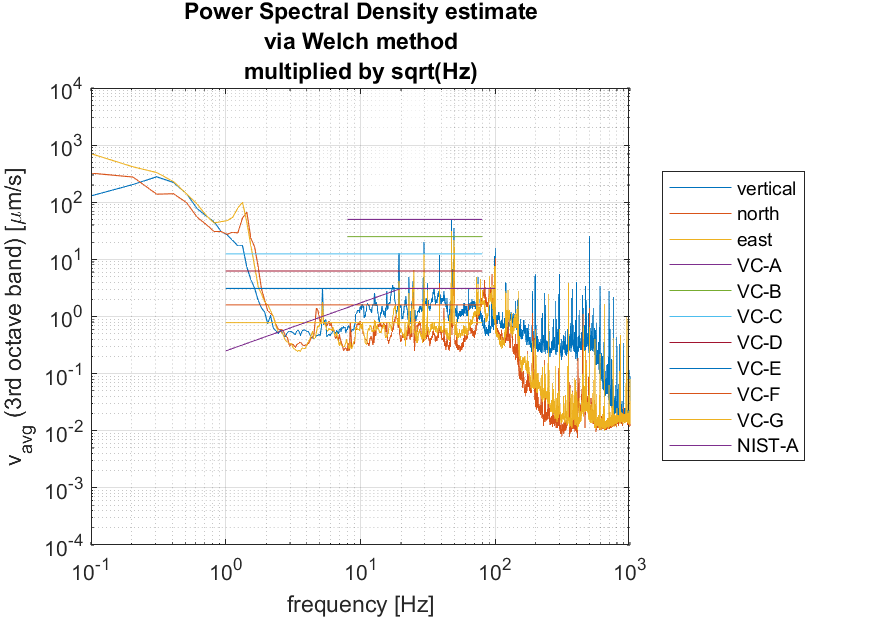
\includegraphics[width=\textwidth]{img/resonance/geophone_measurement_position_1.png}
    \caption{Measured vibration data in the Van der Waals Stacking Facility laboratory on the position of the stacking instrumentation. By J. Scheffer}
    \label{fig:GEOPhone_measurement}
  \end{minipage}
  \hfill
  \begin{minipage}[b]{0.49\textwidth}
    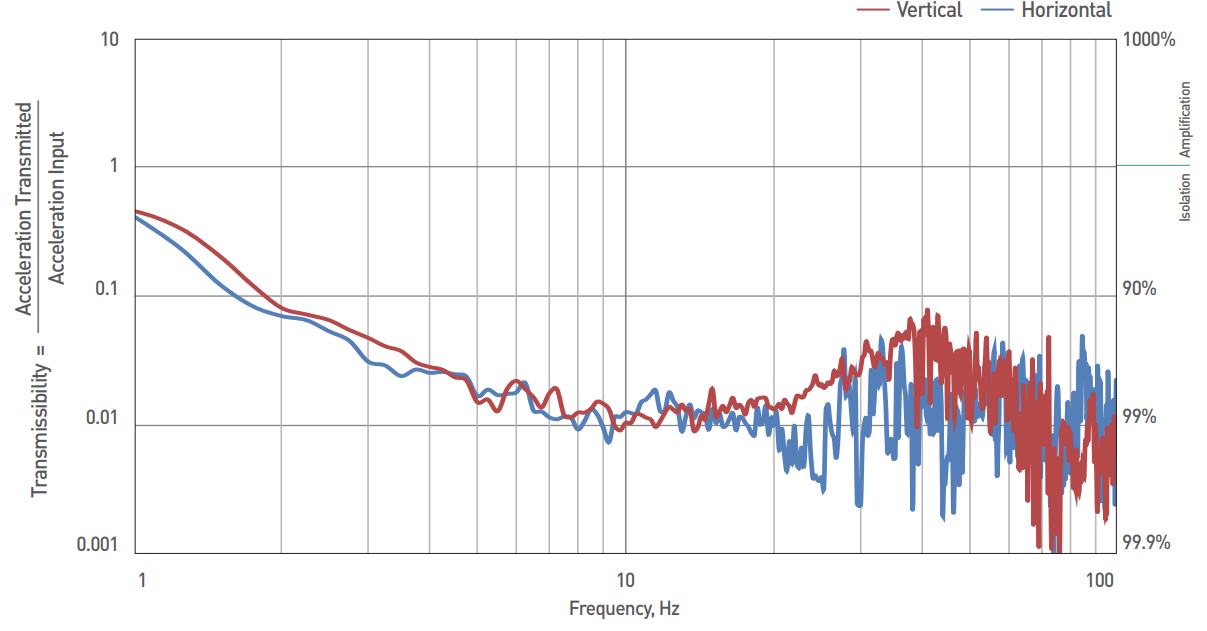
\includegraphics[width=\textwidth]{img/resonance/damping_table_response.png}
    \caption{}
    \label{fig:damp_table_response}
  \end{minipage}
\end{figure}

\todo{uitzoeken aan welke vc norm wij willen voldoen}
\todo{betekenis van NIST-A norm uitzoeken}

\subsection{Criteria}
Door het analyseren vcan de workflow van handmatige en gemotoriseerde commerciele stamping opstellingen in combinatie met literatuur studie is een lijst aan minimale eisen opgesteld waar het te ontwikkelen instrument aan moet voldoen.

\begin{enumerate}[noitemsep]
  \item Mask holder
  \begin{enumerate}[noitemsep]
    \item The mask should be motorized and able to move in the x, y and z direction with a resolution of $>30$ nm.
    \item The pitch of the mask should be able to be adjusted with a resolution of $>0.05^{\circ}$.
    \item The yaw of the mask should be able to be adjusted with a resolution of $>0.05^{\circ}$, with a minimum range of $180^{\circ}$.
  \end{enumerate}
  \item Sample holder
  \begin{enumerate}[noitemsep]
    \item The sample holder should be able to hold a minimum of 2 samples.
    \item The sample should be able to heat with a ramp speed of $2.0 - 50.0^{\circ} C/s$
    \item The sample should be able to cool with a ramp speed of $-0.1 - 30.0^{\circ} C/s$ 
  \end{enumerate}
  \item Microscope \& stand
  \begin{enumerate}[noitemsep]
    \item Due to the fact that the VDWSF laboratry has problems with external vibrations (see \ref{fig:GEOPhone_measurement} the microscope stand should be as rigid as possible to make the instrument behave like one rigid body instead of a system of multiple bodies.
    \item The microscope should a 20x objective with correction collar to be able to focus on the sample through the mask holder glass slide.
  \end{enumerate}


\end{enumerate}

\section{Methods \& Results}
\subsection{Stand design}

Voor het fabriceren van stacks is het belangrijk dat de opstelling zo min mogenlijk beinvloed word door trillingen uit de omgeving. \todo{Verwijzen naar verwachte trillingen grafiek}. Om deze reden is er voor gekozen om in samenwerking met LION FMD een aantal uitwijkings simulaties uit te voeren om een inschatting te kunnen maken over de maximale uitwijking onder een statische kracht van de microscoop stand. 

Het complete instrument bestaat uit verschillende aspecten die in de volgende hoofdstukken behandelt zullen worden. Voor een overzicht van de gebruikte hard- en software componenten zie \ref{fig:software_architecture}. 



\begin{figure}[H]
  \centering
  \begin{minipage}[b]{0.45\textwidth}
    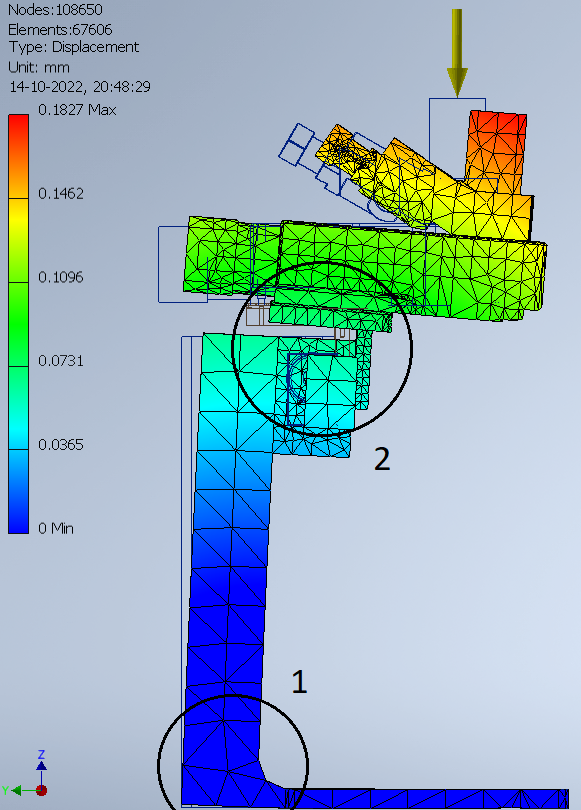
\includegraphics[width=\textwidth]{img/rigidity_simulation/study_4.png}
    \caption{100 N pressing force on a static point on the microscope. To reduce displacement a $30\mathrm{mm}$ fillet was added between the base-plate and stand, reducing the maximum displacent to $183\mathrm{\mu m}$. By R. Stoelwinder }
    \label{fig:disp_study5}
  \end{minipage}
  \hfill
  \begin{minipage}[b]{0.45\textwidth}
    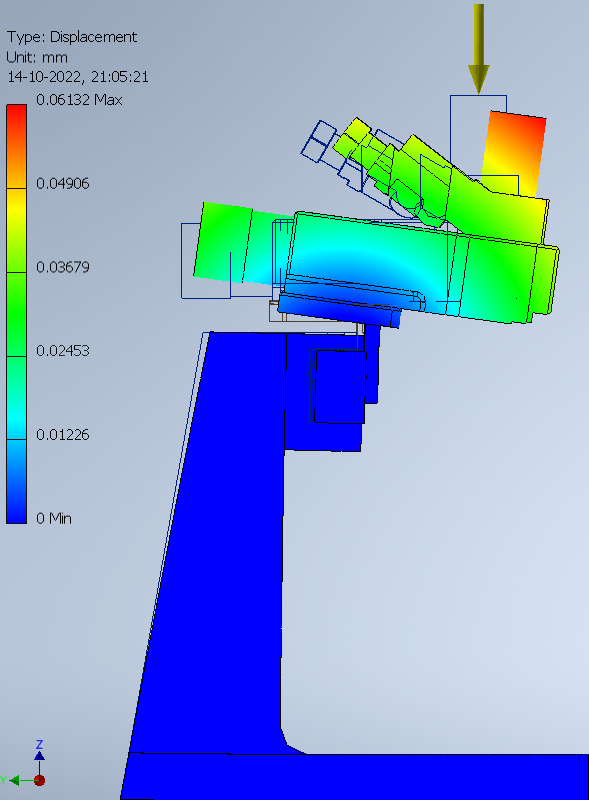
\includegraphics[width=\textwidth]{img/rigidity_simulation/study_7.png}
    \caption{100N pressing force on a static point on the microscope head. To reduce the the maximum displacement the thickness of the base-plate is increased from $20\mathrm{mm}$ to $50\mathrm{mm}$, reducing the maximum displacement to $50\mathrm{\mu m}$. By R. Stoelwinder}
    \label{fig:disp_study7}
  \end{minipage}
\end{figure}

\begin{figure}[H]
  \centering
  \begin{minipage}[b]{0.45\textwidth}
    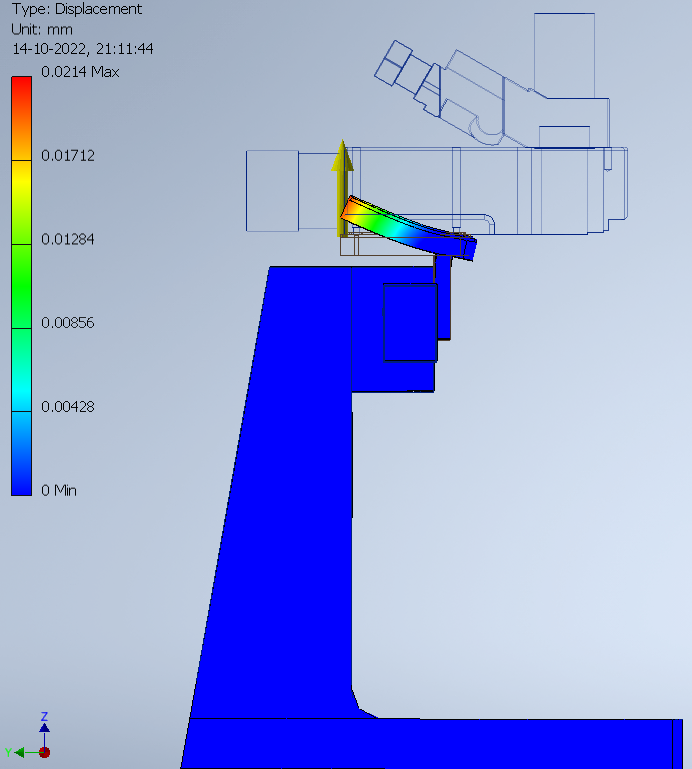
\includegraphics[width=\textwidth]{img/rigidity_simulation/study_8.png}
    \caption{100N pulling force on a static point on the corner plate causing a $21\mathrm{\mu m}$ displacement. By R. Stoelwinder}
    \label{fig:disp_study8}
  \end{minipage}
  \hfill
  \begin{minipage}[b]{0.45\textwidth}
    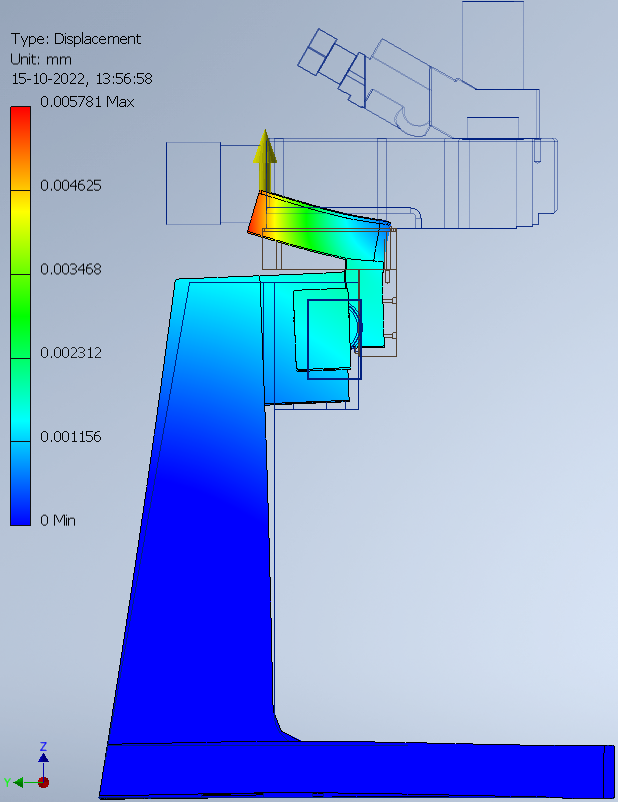
\includegraphics[width=1\textwidth]{img/rigidity_simulation/study_10.png}
    \caption{100 N pulling force on a static point on the corner-plate. To reduce the maximum displacement the thickness of the corner plate is increased from  $20\mathrm{mm}$ to $40\mathrm{mm}$, reducing the maximum displacement to $5\mathrm{\mu m}$. By R. Stoelwinder }
    \label{fig:disp_study10}
  \end{minipage}
\end{figure}

\subsection{Mask design}
the mask consists of two major parts: the mask holder wich holds the stamping polymer and the stages wich are used to position the mask above the sample

For the mask holder 

\todo{CAD schema van de mask holder invoegen}
\begin{figure}[H]
  \centering
  \begin{minipage}[b]{0.45\textwidth}
    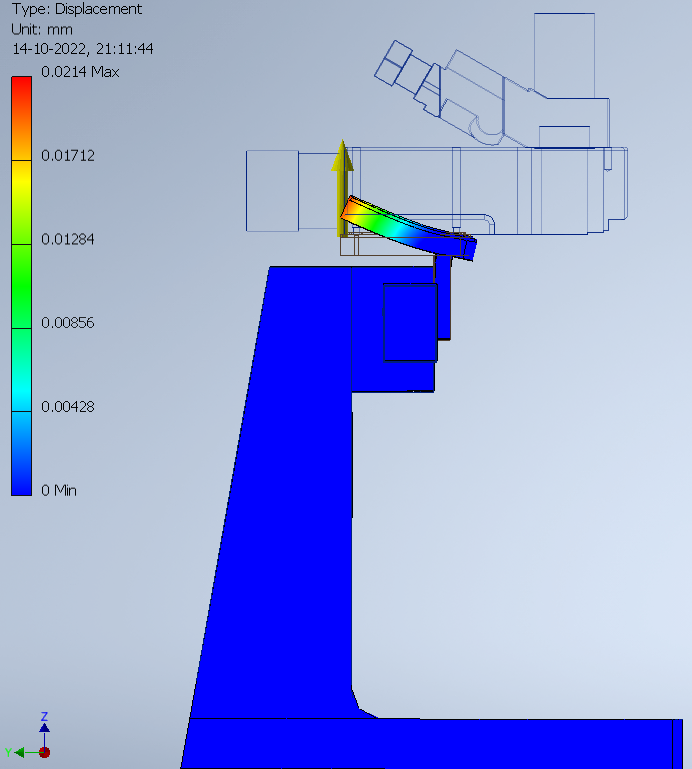
\includegraphics[width=\textwidth]{img/rigidity_simulation/study_8.png}
    \caption{The mask holder schematic. By R. Stoelwinder}
    \label{fig:CAD_mask_holder}
  \end{minipage}
  \hfill
  \begin{minipage}[b]{0.45\textwidth}
    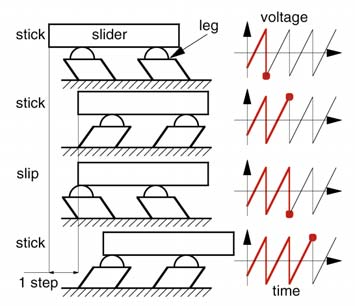
\includegraphics[width=1\textwidth]{img/sample_holder_and_mask/Stick-slip-piezo-actuator-operation-principle.png}
    \caption{Operating principle of a slip-stick actuator mechanism 
    \citep{mazerollePositioningHandlingMeasuring2003}}
    \label{fig:slip_stick_principle}
  \end{minipage}
\end{figure}

\subsection{Sample holder design}

de hoofdtaak van de samplehouder is zoals de naam zegt het in positie houden van het monster waarmee gewerkt word (in dit geval een waver). Net zoals de rest van het instrument is het van belang om de sample houder zo rigide mogenlijk te maken om ervoor te zorgen dat de trillingen van de masker en de camera in fase blijven.

Tijdens de duur van dit project is het eerste prototype van de samplehouder gefabriceerd en zijn de plannen voor het vervolg ontwerp gemaakt. Het prototype (zie figuur \ref{fig:CAD_mask_holder}) bestaat uit 3 onderdelen: Het sample bed, isolatielaag en de dump cilinder. Het sample bed bevat de benodigde componenten om de het sample naar op gewilde temperatuur tussen 0 en 200 graden C krijgen, hiervoor worden een heating coil (verwarmen) en peltier element (koelen) gebruikt. Het samplebed bevat ook een vacuum aansluiting die gebuikt kan worden om het sample stugger te bevestigen wanneer de gebruiker trillingsproblemen ondervind. 

De functie van de isolatielaag is het isoleren van het samplebed en de dump cilinder om te voorkomen dat warmte vanuit de dumpcilinder teruglekt in het sampleblok (van belang tijdens koelen van het monster)

\todo{keuze voor peek en mica onderbouwen}

\todo{CAD schema van de sample holder invoegen}
% Insert the temperature graph and the cad schematic of the sample holder
\begin{figure}[H]
  \centering
  \begin{minipage}[b]{0.45\textwidth}
    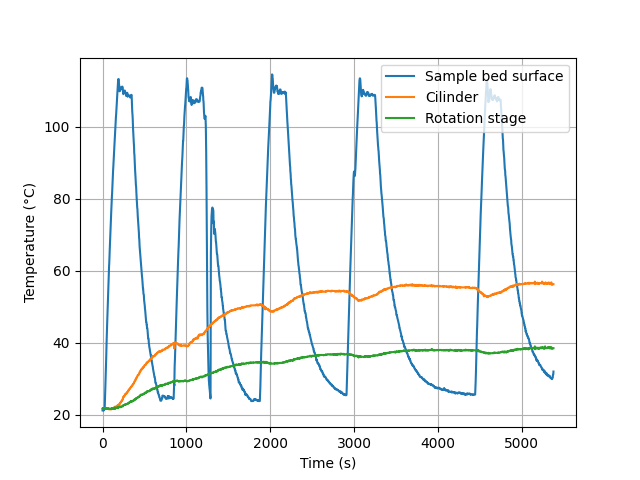
\includegraphics[width=\textwidth]{img/sample_holder_and_mask/temp_cycling.png}
    \caption{Temperature graph of the sample holder when simulating workload by heating to 110 degrees and cooling down to abient temperature (25 degrees) while waiting for 120 seconds when the level is reached}
    \label{fig:temperature_graph}
  \end{minipage}
  \hfill
  \begin{minipage}[b]{0.45\textwidth}
    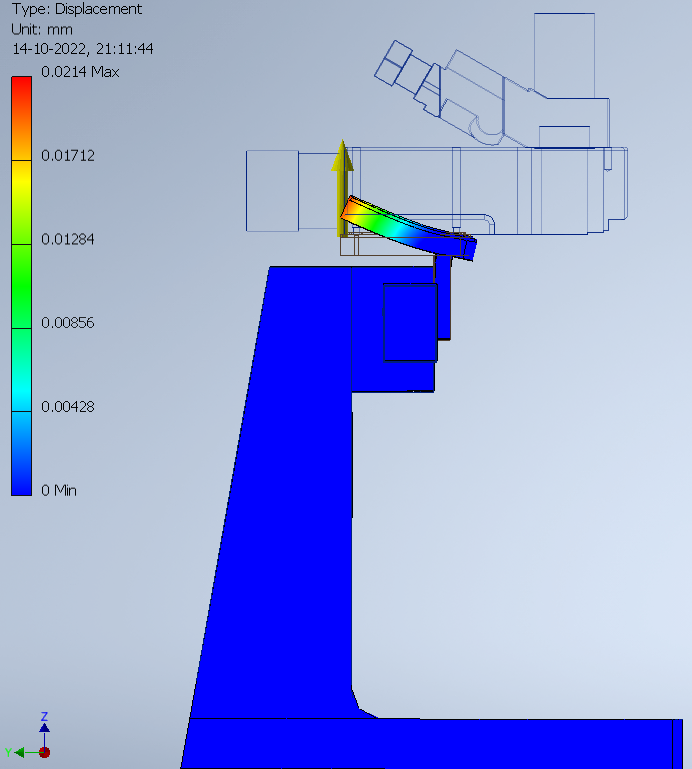
\includegraphics[width=1\textwidth]{img/rigidity_simulation/study_8.png}
    \caption{CAD schematic of the sample holder. By R. Stoelwinder. The sample holder prototype consists of 4 major parts. 1. The sample bed, wich contains a heating coil, peltier element, thermocouple and PT100 sensor. 2. The sample isolation layer. This is a shroud fabricated out of PEEK}
    \label{fig:CAD_sample_holder}
  \end{minipage}
\end{figure}

\subsection{Base stage automisation}

\todo{CAD van bracket invoegen}

for this project the base xy stage (\todo{ref naar optosigma stage invoegen}) has to be automated, this will developed in house in collaboration with LION FMD and ELD. 

The stages were automated using NEMA17 stepper motors \todo{citation invoegen}, and optical endstops.
The stepper motors and endstops are controlled by the controller developed by ELD.
The contents and used tecniques in the controll box are out of the scope for this report.

The first prototype bracket makes it possible to test the complete system and work out implementation bugs. 
It is recommended to create further iterations of the brackes as the current version can flex $\pm 3mm$ and this has a detremental effect on the rigidity of the base xy stage, this because the stages are held in place by the stepper motor. 
Furthermore it is also recommended to replace the ball bearings in the spindles as these were damaged during fabrication and the spindle is now only held in place by the stepper motor

\subsection{Stage calibration}
Due to the mchanisms used in some of the actuators it is not possible to calibrate all the staged,
nor is this needed for the application. 
The stages that cannot be calibrated are the x, y, and z axis of the mask due to the used slip-stick mechanism (see figure \ref{fig:slip_stick_principle}). 

The slip stick mechanism makes it possible to use piezo actuators with high resolution for an unbound range.
The drawback is that due to the slip stick mechanism (friction based) the actuator has a position uncertainty of \todo{positie uncertainty invoegen} and a sstep uncertainty of \todo{step variatie invoegen}.

\subsection{Software}
Because one of the main criteria of the project is flexibility and modularity this has to be taken in consideration from the beginning. 
This means the project needs to be created in a structured and standardised way using design patterns and a modular architecture (see appendix \ref{ap:design_patterns} for the definition of these terms).

\subsubsection{Architecture}
As a main architecture a web application inspired framework is used. 
This means that the system consist of three major components: Frontend, Middleware and backend (for more information about these definitions see appendix \ref{ap:design_patterns}). 
Using standard design patterns makes getting to know the code and editing it less cumbersome and error prone for future developers.
An overview of the system flow can be seen in figure \ref{fig:software_architecture}

\todo{laatste pijlen in de correcte richting zetten}
\begin{figure}[htp]
  \centering
  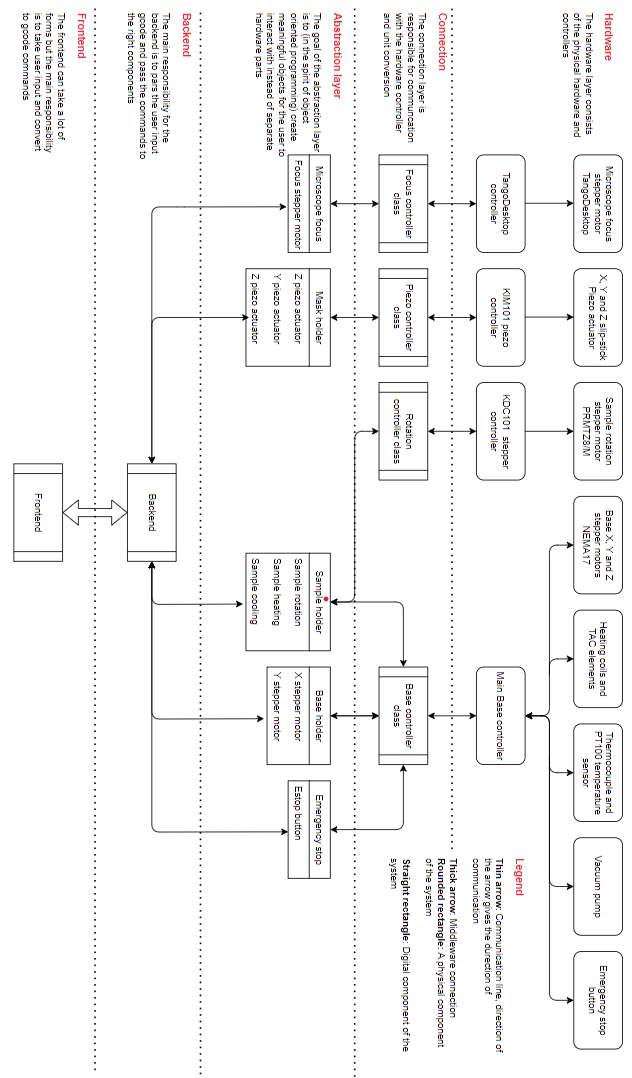
\includegraphics[width=0.8\textwidth]{img/code_flow.png}
  \caption{Software flow of the project.}
  \label{fig:software_architecture}
\end{figure}

\subsubsection{Frontend}
The frontend is the part of the system that is visible to the user.
This part of the system is responsible for the user interface and the communication with the middleware.
The system has two pre made interface options: GUI and TUI.
For operators of the system it is recommended to use the GUI as no knowledge of the command set is needed and safety features like thermal-runaway and forbidden areas are enabled.
For developers it is recommended to use the TUI as it is more flexible and allows for more control over the system.

The GUI is created using QT6 with Pyside6 bindings \todo{citation invoegen} to ensure interoperability between different operating systems and detailed documentation for future developers.

The TUI consists of a simple loop that pushes the gcode commands to the backend and uses a thread to monitor the backend response.

\subsubsection{Middleware}
The middleware is a method that can be used to communicate between the frond and backend. 
The middleware base class (see \ref{ap:middleware_base_class}) contains all the base methods needed for the system to work with a middleware method.
The system contains two default middleware methods: The processing pipe, wich is used for when the backend runs on the same computer as the frondend but on a seperate core (it is strongly discuraged to run the backend on the same core as the frondend as this makes the backend behavoir depend on core workload.) 
The second method is the serial method and is based on the PySerial library \todo{citation invoegen} and is used when the backend runs a differend computer than the frondend.
The serial middleware method can be easily adapted to work with wireless serial communication but this is dicuraged as this method is more prone to errors.

\subsubsection{Backend}
The backend is the part of the system that is responsible for the communication with the hardware and the middleware and managed the object the user can interact with (sample holder, mask holder, etc.)
The backend accepts all classes that inherit from their respective base class and abide the programming guidelines \todo{referentie naar docs toevoegen}

Due to time constraints it was not possible to develop the backend to run on unix based systems

\todo{stukje over FTDI issue tovoegen}
\todo{stukje over voordeel van runnen op IO controller toevoegen}

\subsubsection{Forbidden areas}
To prevent the system from damaging itself or the sample it is important to prevent the system from moving to certain areas in certain states.

Phase space variables (system attributes):
\begin{itemize}
    \item Position of all the axis*
    \item Velocity of all the axis
    \item Acceleration of all the axix
    \item Sample temperature
    \item Sample heating and cooling ramp
\end{itemize}

This means the phase space will consist of 21 dimensions, where each dimension reperesents the current value of a system attribute.

First the phase space is bordered off by the hardware limitations like maximum velocity, minmal reproducable step size, range, etc.
Further forbidden areas are studied using a fractional factorial design to determine the most important variables that influence the system.

The forbidden areas will be determined using a fractional factorial design with the following parameters

(see excel file)




\clearpage
\section{Conclusion}

\section{Discussion}


\newpage
\bibliographystyle{abbrvnat}
\bibliography{References}

\clearpage
\appendix

\section{Programming terms}
\label{ap:programming_terms}
\subsection*{Design patterns}
\label{ap:design_patterns}
In programming, a design pattern is a general repeatable solution to a commonly occurring problem in software design. 
A design pattern is not a finished design that can be transformed directly into code. 
It is a description or template for how to solve a problem that can be used in many different situations.\\

Design patterns are used to describe solutions to specific design problems in object-oriented programming. 
They provide a way to reuse successful designs and design solutions that have been proven to work well in the past.\\

There are many different types of design patterns, including creational patterns, structural patterns, and behavioral patterns. 
Creational patterns deal with object creation mechanisms, trying to create objects in a manner suitable to the situation. 
Structural patterns deal with object composition, creating relationships between objects to form larger structures. 
Behavioral patterns focus on communication between objects, what goes on between objects and how they operate together.\\

Using design patterns can make it easier to design and develop software, because they provide a common vocabulary and framework for thinking about and solving design problems. 
They also help to make code more maintainable and scalable by providing a clear, consistent way to structure and organize it.\\

\subsection*{Modular architecture}
\label{ap:modular_architecture}
In a web application or system, the frontend refers to the part of the application that the user interacts with, typically through a web browser. 
It includes all the elements that the user can see and interact with, such as the layout, user interface, and visual design of the application.\\

The backend, on the other hand, refers to the part of the application that handles the logic and processing behind the scenes. 
It is responsible for tasks such as storing and retrieving data from a database, performing calculations and processing, and interacting with other systems or APIs.\\

Middleware is software that sits between the frontend and the backend and helps to facilitate communication and data exchange between them. 
It can provide functions such as authentication, routing, and data transformation, and can help to abstract away some of the complexity of the backend from the frontend.\\

In a web application, the frontend and backend are typically implemented using different technologies and run on different servers or infrastructure. 
Middleware can be implemented using a variety of technologies, depending on the specific requirements of the application.\\

\subsection*{Multi-threading and processing}
\label{ap:multi_threading_and_processing}
In computer science, multi-threading is a technique that allows a single process or program to have multiple threads of execution. 
A thread is a separate flow of execution within a process, and each thread can run concurrently or in parallel with the other threads within the same process.\\

Multi-threading can be used to improve the performance of a program by allowing it to perform multiple tasks concurrently. 
For example, a program that has a user interface and needs to perform some time-consuming calculations in the background could use multi-threading to allow the user to continue interacting with the interface while the calculations are being performed.\\

Multi-processing is a technique that allows a computer to run multiple processes simultaneously. A process is an instance of a program that is being executed by the operating system. Each process has its own memory space and runs in a separate environment, and multiple processes can be run concurrently on different cores or processors within a computer.\\

Multi-processing can be used to improve the performance of a program by allowing it to take advantage of multiple processors or cores within a computer. 
This can be particularly useful for programs that need to perform a lot of calculations or that are designed to run on a distributed system with multiple machines.\\

\clearpage
\section{Backend base classes}
The base classes are used as a template for new components. The base classes contain all the functions that are required for the component to work with the rest of the system. Notice that two different errors can be raised: NotImplementedError and NotSupportedError. The functions that raise a NotImplementedError should always be implemented for the component to work correctly with the rest of the system. It is safe to raise NotSupportedError as these are caught and handled by the system.

\label{ap:backend_base_classes}
\subsection*{Harware base class}
\label{ap:hardware_base_class}
\lstinputlisting[language=Python]{code/backend/hardware_base.py}

\clearpage
\subsection*{Middleware base class}
\label{ap:middleware_base_class}
\lstinputlisting[language=Python]{code/backend/middleware_base.py}


%\printbibliography

%\clearpage
%\section*{Appendix}



%\begin{figure}[H]
%  \centering
%  \begin{minipage}[b]{0.4\textwidth}
%    \includegraphics[width=\textwidth]{img/plot3.png}
%    \caption{ROC Curve: Random Plot 2}
%    \label{fig:Wrong_Orientation}
%  \end{minipage}
%  \hfill
%  \begin{minipage}[b]{0.4\textwidth}
%    \includegraphics[width=\textwidth]{img/plot4.png}
%    \caption{ROC Curve: Random Plot 2}
%    \label{fig:Unusual}
%  \end{minipage}
%\end{figure}

%****** Extra package work if needed
% To add math, use
%\begin{equation}
 %Helpful links    https://www.overleaf.com/learn/latex/Mathematical_expressions
%\end{equation}

%To add hyperlinks, use 
%For further references see \href{http://www.overleaf.com}{Something Linky} or go to the next url: \url{http://www.overleaf.com}

% It's also possible to link directly any word or \hyperlink{thesentence}{any sentence} in you document.

% Tables 

% \begin{table}[h!]
% \centering
%  \begin{tabular}{||c c c c||} 
%  \hline
%  Col1 & Col2 & Col2 & Col3 \\ [0.5ex] 
%  \hline\hline
%  1 & 6 & 87837 & 787 \\ 
%  2 & 7 & 78 & 5415 \\
%  3 & 545 & 778 & 7507 \\
%  4 & 545 & 18744 & 7560 \\
%  5 & 88 & 788 & 6344 \\ [1ex] 
%  \hline
%  \end{tabular}
% \end{table}

% Images

% upload your images to the img folder. To print them in the document, uncomment the following
% \begin{figure}[h]
%     \centering
%     \includegraphics[width=0.25\textwidth]{/img/YourImageTitle}
%     \caption{a nice plot}
%     \label{fig:mesh1}
% \end{figure}

% As you can see in the figure \ref{fig:mesh1}, the 
% function grows near 0. Also, in the page \pageref{fig:mesh1} 
% is the same example.

\clearpage
\todototoc
\listoftodos
\end{document}
